\documentclass[12pt, a4paper, titlepage]{article}
\usepackage[a4paper,top=2.5cm,bottom=2cm,left=2cm,right=2cm]{geometry}
\usepackage[english]{babel}
\usepackage[hidelinks]{hyperref}
\usepackage{multirow, graphicx}
\usepackage{algorithm}
\usepackage{capt-of}
\usepackage{amsmath}
\usepackage{longtable}
\usepackage{caption}
\usepackage{booktabs}
\usepackage{algpseudocode}
\usepackage{makecell}
\usepackage[utf8]{inputenc}
\usepackage{fixltx2e}
\usepackage{listings}
\usepackage{hyperref}
\usepackage{makecell}
\usepackage{changepage}
\usepackage{paracol}
\usepackage{siunitx}
\usepackage{lipsum}
\usepackage[swapnames]{frontespizio}
\usepackage{fancyhdr}
\usepackage{lastpage}
\usepackage{pdfpages}
\usepackage{tabularx, pbox}
\usepackage{subcaption}
\usepackage[toc, acronym, nonumberlist, automake]{glossaries}
\usepackage{pgfgantt}
\usepackage{tcolorbox}
\usepackage{footmisc}
\usepackage{colortbl}

%\renewcommand{\thesection}{\thechapter.\number\numexpr\value{section}-1\relax}
%\renewcommand{\thesubsection}{\thesection.\number\numexpr\value{subsection}-1\relax}
%\renewcommand{\thesubsubsection}{\thesubsection.\number\numexpr\value{subsubsection}-1\relax}
\setcounter{secnumdepth}{3}
	
\makeglossaries	

%Glossary

\newglossaryentry{word}{name=Microsoft Word, description={is a word processor published by Microsoft. It is one of the office productivity applications included in the Microsoft Office suite.\cite{wikipedia}}}

\newglossaryentry{pp}{name=Microsoft PowerPoint, description={is a presentation program, published by Microsoft. It is one of the office productivity applications included in the Microsoft Office suite.\cite{wikipedia}}}

\newglossaryentry{teams}{name=Microsoft Teams, description={is a business communication platform, published by Microsoft. It is one of the office productivity applications included in the Microsoft Office suite.\cite{wikipedia}}}

\newglossaryentry{drive}{name=Microsoft OneDrive, description={is a file hosting service and synchronization service, published by Microsoft. It is one of the office productivity applications included in the Microsoft Office suite.\cite{wikipedia}}}

\newglossaryentry{outlook}{name=Microsoft Outlook, description={is s a personal information manager web app from Microsoft consisting of webmail, calendaring, contacts, and tasks services. It is one of the office productivity applications included in the Microsoft Office suite.\cite{wikipedia}}}

\newglossaryentry{office}{name=Microsoft Office, description={is a family of client software, server software, and services developed by Microsoft.\cite{wikipedia}}}

\newglossaryentry{kb}{name=Knowledge Base, description={a place for creating, sharing, using and managing the knowledge and information of an organization.\cite{wikipedia}}}

\newglossaryentry{anonymous}{name=Anonymous, description={is a decentralized international activist/hacktivist collective/movement that is widely known for its various cyber attacks against several governments, government institutions and government agencies, corporations, and the Church of Scientology.\cite{wikipedia}}}

\newglossaryentry{repository}{name=Repository, description={,in revision control systems, is a data structure that stores metadata for a set of files or directory structure.\cite{wikipedia}}}

%Glossary Acronyms entry

\newglossaryentry{slag}{name=Service-level Agreement, description={is a commitment between a service provider and a client. Particular aspects of the service {–} quality, availability, responsibilities {–} are agreed between the service provider and the service user.\cite{wikipedia}}}

\newglossaryentry{pstng}{name=Public switched telephone network, description={the aggregate of the world's circuit-switched telephone networks that are operated by national, regional, or local telephony operators, providing infrastructure and services for public telecommunication.\cite{wikipedia}}}

\newglossaryentry{cccg}{type=\glsdefaulttype, name=Chaos Computer Club, description={is Europe's largest association of hackers with 7700 registered members.\cite{wikipedia}}}

\newglossaryentry{iacg}{type=\glsdefaulttype, name=Infrastructure as Code, description={is the process of managing and provisioning computer data centers through machine-readable definition files, rather than physical hardware configuration or interactive configuration tools.\cite{wikipedia}}}

\newglossaryentry{hag}{type=\glsdefaulttype, name=High Availability, description={is a characteristic of a system which aims to ensure an agreed level of operational performance, usually uptime, for a higher than normal period.\cite{wikipedia}}}

\newglossaryentry{mdmg}{type=\glsdefaulttype, name=Mobile device management, description={is typically a deployment of a combination of on-device applications and configurations, corporate policies and certificates, and backend infrastructure, for the purpose of simplifying and enhancing the IT management of end user devices.\cite{wikipedia}}}

\newglossaryentry{adg}{type=\glsdefaulttype, name=Active Directory, description={ is a directory service developed by Microsoft for Windows domain networks. It is included in most Windows Server operating systems as a set of processes and services. Initially, Active Directory was used only for centralized domain management. However, Active Directory eventually became an umbrella title for a broad range of directory-based identity-related services.\cite{wikipedia}}}

\newglossaryentry{polpg}{name=Principle of least privilege, description={ also known as the principle of minimal privilege or the principle of least authority, requires that in a particular abstraction layer of a computing environment, every module (such as a process, a user, or a program, depending on the subject) must be able to access only the information and resources that are necessary for its legitimate purpose.\cite{wikipedia}}}

\newglossaryentry{itilg}{name=Information Technology Infrastructure Library, description={is a set of detailed practices for IT activities that describes processes, procedures, tasks, and checklists which are neither organization-specific nor technology-specific, but can be applied by an organization toward strategy, delivering value, and maintaining a minimum level of competency.\cite{wikipedia}}}

\newglossaryentry{mttrg}{name=Mean time to repair, description={is a basic measure of the maintainability of repairable items. It represents the average time required to repair a failed component or device. Expressed mathematically, it is the total corrective maintenance time for failures divided by the total number of corrective maintenance actions for failures during a given period of time.\cite{wikipedia}}}

\newglossaryentry{iscedg}{name=International Standard Classification of Education, description={is a statistical framework for organizing information on education maintained by the \textit{\gls{unesco}}. It is a member of the international family of economic and social classifications of the United Nations.\cite{wikipedia}}}

\newglossaryentry{cefrg}{name=Common European Framework of Reference for Languages, description={is a guideline used to describe achievements of learners of foreign languages across Europe and, increasingly, in other countries. The CEFR is also intended to make it easier for educational institutions and employers to evaluate the language qualifications of candidates to education admission or employment.\cite{wikipedia}}}

%Acronyms

\newglossaryentry{perc}{type=\acronymtype, name={PERC}, description={The Propane Education \& Research Council}}

\newglossaryentry{smart}{type=\acronymtype, name={S.M.A.R.T.}, description={Specific, Measurable, Achievable, Relevant and Time-based}}

\newglossaryentry{etz}{type=\acronymtype, name={ETZ}, description={Eastern Time Zone}}

\newglossaryentry{st}{type=\acronymtype, name={S\&T}, description={Sales and Training}}

\newglossaryentry{api}{type=\acronymtype, name={API}, description={Application Programming Interface}}

\newglossaryentry{fifo}{type=\acronymtype, name={FIFO}, description={First In, First Out}}

\newglossaryentry{raci}{type=\acronymtype, name={RACI}, description={Responsible Accountable Consulted Informed}}

\newglossaryentry{vm}{type=\acronymtype, name={VM}, description={Virtual Machine}}

\newglossaryentry{msp}{type=\acronymtype, name={MSP}, description={Managed Service Provider}}

\newglossaryentry{unesco}{type=\acronymtype, name={UNESCO}, description={United Nations Educational, Scientific and Cultural Organization}}

\newglossaryentry{rfp}{type=\acronymtype, name={RFP}, description={Request for Proposal}}

\newglossaryentry{pm}{type=\acronymtype, name={PM}, description={Post meridiem}}

\newglossaryentry{am}{type=\acronymtype, name={AM}, description={Ante meridiem}}

%Acronyms glossary entry

\newglossaryentry{sla}{type=\acronymtype, name={SLA}, description={Service-Level Agreement}, first={SLA\glsadd{slag}}, see=[Glossary:]{slag}}

\newglossaryentry{pstn}{type=\acronymtype, name={PSTN}, description={Public switched telephone network}, first={PSTN\glsadd{pstng}}, see=[Glossary:]{pstng}}

\newglossaryentry{ccc}{type=\acronymtype, name={CCC}, description={Chaos Computer Club}, first={CCC\glsadd{cccg}}, see=[Glossary:]{cccg}}

\newglossaryentry{iac}{type=\acronymtype, name={IaC}, description={Infrastructure as Code}, first={IaC\glsadd{iacg}}, see=[Glossary:]{iacg}}

\newglossaryentry{ha}{type=\acronymtype, name={HA}, description={High Availability}, first={HA\glsadd{hag}}, see=[Glossary:]{hag}}

\newglossaryentry{ad}{type=\acronymtype, name={AD}, description={Active Directory}, first={AD\glsadd{adg}}, see=[Glossary:]{adg}}

\newglossaryentry{mdm}{type=\acronymtype, name={MDM}, description={Mobile device management}, first={MDM\glsadd{mdmg}}, see=[Glossary:]{mdmg}}

\newglossaryentry{polp}{type=\acronymtype, name={PoLP}, description={Principle of least privilege}, first={PoLP\glsadd{polpg}}, see=[Glossary:]{polpg}}

\newglossaryentry{itil}{type=\acronymtype, name={ITIL}, description={Information Technology Infrastructure Library}, first={ITIL\glsadd{itilg}}, see=[Glossary:]{itilg}}

\newglossaryentry{mttr}{type=\acronymtype, name={MTTR}, description={Mean time to repair}, first={MTTR\glsadd{mttrg}}, see=[Glossary:]{mttrg}}

\newglossaryentry{isced}{type=\acronymtype, name={ISCED}, description={United Nations Educational, Scientific and Cultural Organization}, first={ISCED\glsadd{iscedg}}, see=[Glossary:]{iscedg}}

\newglossaryentry{cefr}{type=\acronymtype, name={CEFR}, description={Common European Framework of Reference for Languages}, first={CEFR\glsadd{cefrg}}}


	
\begin{document}

\newcommand{\HRule}{\rule{\linewidth}{0.5mm}}
\pagenumbering{gobble}

\begin{center}

	\textsc{\LARGE Università degli Studi di Padova}\\[1cm]

	
\includegraphics[height=5cm]{img/UniPd.png}\\[1cm]

	
\includegraphics[height=1.5cm, width = 9cm]{img/MathDip.png}\\
	\textsc{Dipartimento di Matematica ``Tullio Levi-Civita''}\\[1.2cm]
	\textsc{\Large Scuola di Scienze}\\[0.5cm]

	\textsc{\large Corso di Laurea Magistrale in Informatica}\\[0.5cm]

	\vspace{2.5cm}


	\HRule \\[0.4cm]
	{ \huge \bfseries Response to a Request for Proposal }\\[0.4cm]
	\HRule \\[1.5cm]


	\vspace{2.5cm}


	{\large
		Francesco Antonio Migliorin \\
		1207422 \\
		Anno 2020/2021}\\[2cm]


	\vfill
\end{center}

\includepdf[pages={1}]{./sections/cover-letter.pdf}
\renewcommand{\arraystretch}{2.7}
\section*{Proposal Cover Sheet}
\begin{table}[H]
	\centering 
	\begin{tabularx}{\linewidth}{|XX|}
		\hline
		\textbf{Giglium Proposal Code}  &    GGL-RFP-V1.0{-}2021\\
		\textbf{Technical Areas}: & Help desk, communication improvements, and customer satisfaction  \\
		\textbf{Proposal Title} & Request for Proposals for the Development and
		Support of the CETP e-learning Help Desk \\
		\textbf{Lead Organization} & Giglium, Inc.\ \makecell{Via Trieste 63 35132 Padova (PD)}\\
		\textbf{Technical Point of Contact} & Mario Rossi Giglium, Inc.\ \makecell{Via Trieste 63 35132 Padova (PD)} \makecell{Phone: 123 456 7890} \makecell{Email: mario.rossi@giglium.com}\\
		\textbf{Administrative Point of Contact} & Francesco Antonio Migliorin Giglium, Inc.\ \makecell{Via Trieste 63 35132 Padova (PD)} \makecell{Phone: 123 456 7890} \makecell{Email: francesco.migliorin@giglium.com}\\
		\textbf{Proposal Validity Period} & \today\text{ to }December 31, 2021 \\
		\textbf{Date Proposal Submitted} & \today \\
		\hline
	\end{tabularx}
\end{table}
\renewcommand{\arraystretch}{1}
\newpage
\setcounter{tocdepth}{2}
\tableofcontents
\newpage
\listoffigures
\newpage
\listoftables
\setcounter{table}{0}
\pagestyle{fancy}
\fancyhf{}
\rhead{Response to a RFP}
\lhead{IT Management Course}
\cfoot{\thepage}
\clearpage
\pagenumbering{arabic}
\section{Introduction}\label{introduction}
\gls{perc} is a non-profit organization
authorized by the Propane Education and Research Act of 1996, Public Law 104{-}284.
\gls{perc} was created \textit{“to enhance consumer and employee safety and training, to provide for research and development of clean and efficient propane utilization equipment, and to inform and
	educate the public about safety and other issues associated with the use of propane.”} The Certified Employee Training Program has been the \textit{“gold standard”} of training in the
propane industry for several years. To date, this training has been conducted in a classroom
environment using printed books. After a course, students have the option to sit
for a proctored certification exam, overseen by the National Propane Gas Association.
Now the Certified Employee Training Program is developing an e-learning format of this program to release in 2021.\gls{perc} wants to create and Help Desk, to help their students to face all the possible new challenges.

Switching from the traditional classroom and face-to-face instructor training to computer-based training in a virtual classroom makes the learning experience entirely different for students. Their weak monitors make it hard to follow the course and their learning experience becomes problematic. Moreover, most of them find it difficult to keep in tune with the technical requirements of the chosen course. Also, the lack of computer literacy is a major issue among students today. Many of them cannot operate basic programs such as \textit{\gls{word}}\footnote{From here on, all words in italics will indicate a word in the glossary. You can consult the glossary for more information on that word, concept, or product.} and \textit{\gls{pp}} and therefore are not able to handle their files. Furthermore, many students find fixing basic computer problems troublesome, as they do not know this area. However, technological proficiency is a must for following online courses, as it enables students to manage their assignments and courseware in an organized manner without struggling.

Giglium's leadership thanks to this project will change this state of affairs, socially and technically. On the social front, Giglium will facilitate communication with students and help the troubleshooting process to be quicker thanks to the excellent expert teams brought together by us. On the technical side, Giglium will be the editor and, when necessary, author, of a set of rigorous engineering artifacts fit for refinement into a help desk system. Giglium believes that it will be the social and technical catalyst and glue to keep the project lively, on track, and ensure that it meets the expectations of \gls{perc}.


\begin{figure}[ht!]
	\centering
	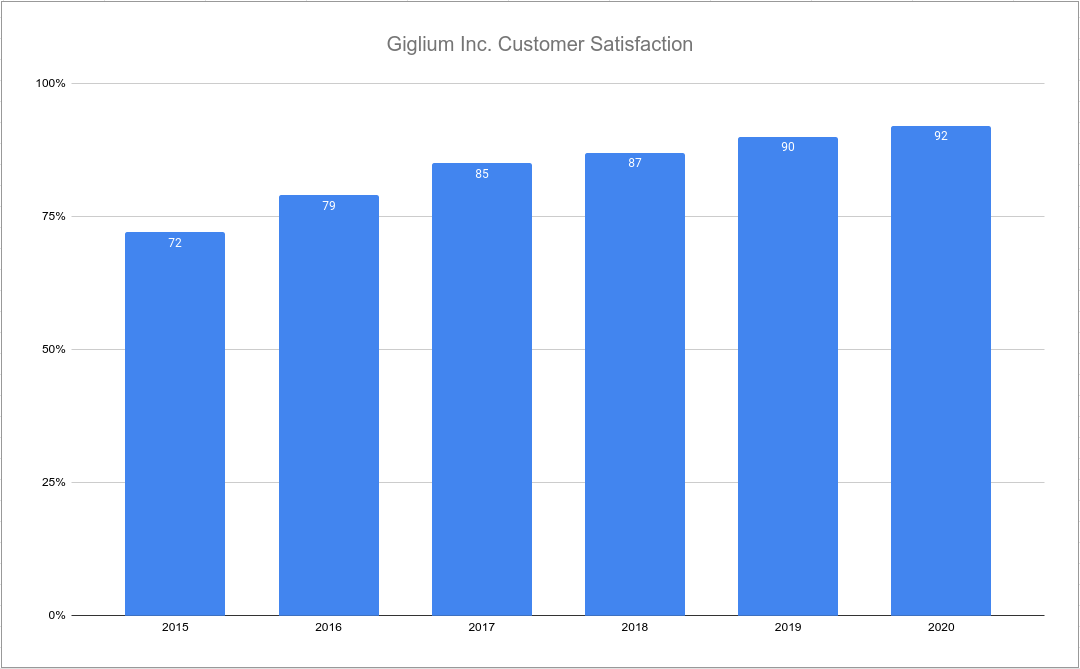
\includegraphics[width=100mm]{./img/introduction/customer-satisfaction-graph.png}
	\caption{Customer Satisfaction: A Giglium Inc.\ Priority}\label{fig:customer-satisfaction}
\end{figure}

\clearpage
The main reasons that Giglium has this belief are multiple. Each year, we hire a third-party research firm to survey hundreds of Giglium customers
worldwide. They are asked what we are doing well and where we need to improve. In Figure~\ref{fig:customer-satisfaction}, as you can see, since we began formally tracking this data, our numbers are strong. In 2020, we reached a possible customer satisfaction score of 92\% out of a possible 100\%, this result was possible since we believe that customers drive our company. And we also believe that we can never be “too close to a customer's needs” or be “listening too much.” It is through our customers that we identify and capture market transitions, measure our success, and design and create solutions. Our customer-centric approach, combined with our culture, is what makes us a “vendor of choice.” Now, at a time when the technology industry is going through a period of dramatic change, Giglum works with the market leader in multiple areas. 
Thanks to this ecosystem of partners, we have earned the trust and satisfaction of our
customers.  

\begin{figure}[ht!]
	\begin{subfigure}{\linewidth}
		
\includegraphics[width=.25\linewidth]{./img/introduction/azure.png}\hfill
		
\includegraphics[width=.25\linewidth]{./img/introduction/gcp.png}\hfill
		
\includegraphics[width=.25\linewidth]{./img/introduction/red-hat.png}
	\end{subfigure}\par\medskip
	\begin{subfigure}{\linewidth}
		
\includegraphics[width=.25\linewidth]{./img/introduction/github.png}\hfill
		
\includegraphics[width=.25\linewidth]{./img/introduction/hashicorp.png}\hfill
		
\includegraphics[width=.25\linewidth]{./img/introduction/jabra.png}
	\end{subfigure}\par\medskip
	\begin{subfigure}{\linewidth}
		
\includegraphics[width=.25\linewidth]{./img/introduction/libraesva.png}\hfill
	\end{subfigure}
	\caption{Giglium, inc.\ partner ecosystem}\label{fig:partner}
\end{figure}

All of these partners are what make Giglium an ideal systems integrator and partner for your digital transformation.

\clearpage
\section{Project Overview}\label{project-overview}
Successfully ensuring that this project meets its goals is critically dependent upon the quality of the project management.

\subsection{PERC's Requisites}
From the \textit{\gls{perc}} \textit{\gls{rfp}} Giglium indentify these mandatory requisites.\footnote{Mandatory requirements will be referred with \texttt{M}, binding as the primary objective required}

\begin{table}[H]
	\centering
	\begin{tabular}{|l|l|} 
		\hline
		\textbf{Code} & \textbf{Description} \\
		\hline
		\texttt{M01} & \parbox{15 cm}{Help desk support from Monday through Friday, 9:00 \textit{\gls{am}} to 9:00 \textit{\gls{pm}} \textit{\gls{etz}}.} \\
		\hline
		\texttt{M02} & \parbox{15 cm}{Student should be able to contact the help desk via a toll-free number~(s), a regular long distance number, email, and fax.} \\
		\hline
		\texttt{M03} & \parbox{15 cm}{Describe in detail the physical locations and arrangement of staff (call center vs.\ home-based).} \\
		\hline
		\texttt{M04} & \parbox{15 cm}{each call will need to be databased in either a new or existing database. If it is a new database Portions of this database may need to be searchable on the \gls{st} Online Resource~\cite{propanesafety}.} \\
		\hline
		\texttt{M05} & \parbox{15 cm}{\textit{\gls{perc}} will provide application-specific scripts for staff.} \\
		\hline
		\texttt{M06} & \parbox{15 cm}{\textit{\gls{perc}} will host the web-based database internally.} \\
		\hline
	\end{tabular}
	\caption{Mandatory requirements}\label{tab:m_requirements}
\end{table}
\noindent From the \textit{\gls{perc}} \textit{\gls{rfp}} Giglium indentify these optional requisites.\footnote{Optional requirements will be referred with \texttt{O}, non-binding or strictly necessary requirements but they representing added value}

\begin{table}[H]
	\centering
	\begin{tabular}{|l|l|} 
		\hline
		\textbf{Code} & \textbf{Description} \\
		\hline
		\texttt{O01} & \parbox{15 cm}{Help desk support considering other types of hours offerings (e.g. 24{-}7, with weekends vs.\ without weekends.)} \\
		\hline
		\texttt{O02} & \parbox{15 cm}{A call queue is preferred.} \\
		\hline
		\texttt{O03} & \parbox{15 cm}{The proposed solution must be scalable to meet increased or decreased demand.} \\
		\hline
	\end{tabular}
	\caption{Optional requirements}\label{tab:o_requirements}
\end{table}

\subsection{PERC's Role}
\textit{\gls{perc}}, via their support team of experts, will act as the expert team. The experts are responsible for making timely and appropriate contributions within their areas of expertise including, but not limited to:

\begin{itemize}
	\item contributions to dialog via email and telephone, online, and face-to-face meeting to help the students with their needs;
	\item the authoring of specific subsections of articles of the \textit{\gls{kb}};
	\item periodically review articles of the \textit{\gls{kb}};
	\item potentially providing feedback on, or editing drafts of the \textit{\gls{kb}};
	\item potentially contributing engineering expertise to the design and development of supporting technical artifacts;
\end{itemize}

It is to be expected that many experts will not have the resources to take a leading role
in the authoring of either the \textit{\gls{kb}} or its supporting artifacts.
Consequently, those aspects of the project are mentioned as potential, rather than mandatory
contributions above.

\subsection{Giglium's Role}
The main technical project management role of Giglium is to facilitate communication with students and help the troubleshooting process to be quicker.

Activities for which Giglium is responsible include, but are not limited to:
\begin{itemize}
	\item creating, triaging, updating, and ensuring the resolution of tickets relating to service requests and incidents;
	\item create and maintain the help desk ticketing system;
	\item helping organize and conduct online, telephone, and face-to-face meetings with students if needed
\end{itemize}
This technical management capacity is complemented by Giglium's role in concretizing the high-level specification of the help desk system described in this proposal. More specifically, Giglium will be the editor and, when necessary, author, of a set of rigorous engineering artifacts fit for refinement into a working help desk system. The expected nature
of these specifications is discussed later in section~\ref*{implementation}.

\subsection{Giglium's Team}
Giglium will gather a team of professionals to meet the needs of \textit{\gls{perc}}, the professional figures are as follows:
\begin{itemize}
	\item \textbf{Solution Architect}: Mario Rossi (\href{mailto:mario.rossi@giglium.com}{mario.rossi@giglium.com}) is the designated solution architect for this project. Mario has many years of experience in this role and several certifications:
	\begin{itemize}
		\item Azure solution Architect\cite{azure_solution_architect_certification};
		\item Sysaid Certification Program\cite{sysaid_certification};
		\item \textit{\gls{itil}} strategic leader\cite{itil_strategic_certification};
		\item Cambridge English qualification C2 proficiency\cite{c2_certification}.
	\end{itemize}
	His task was to design the solution described in section~\ref{implementation} and it will be in charge to analyze and understand the needs of the \textit{\gls{perc}} to adjust the solution that aims at the maximum result with the minimum effort and suit the \gls{perc} needs;
	
	\item \textbf{Cloud Native Developer}: They are the figure responsible for the development of what Mario has designed, in the section~\ref{implementation}. They are experts in their sector and they prove it through certifications:
	\begin{itemize}
		\item Azure Administrator Associate\cite{azure_administrator_certification} or/and Terraform\cite{terraform_associate_certification}\footnote{The final team will be defined after the sign of the proposal.};
		\item \textit{\gls{itil}} v4 foundation\cite{itil_foundation_certification}.
	\end{itemize}
	\item \textbf{Help Desk Coordinator}: It will be the person in charge of enforcing and maintain the procedures described in the section~\ref{procedures}. It will provide first-level assistance, working together with the Help Desk Operator and it will also take care of the communication and the reporting with \textit{\gls{perc}}. To ensure the  service quality and prove its knowledge of the processes, this figure will have the following certification:
	\begin{itemize}
		\item \textit{\gls{itil}} v4 foundation\cite{itil_foundation_certification}.
	\end{itemize}
	\item \textbf{Help Desk Operator}: it will be the operator who will provide the first-level assistance. Giglium  will provided operators with a \textit{\gls{isced}} level greater than or equal to three.
\end{itemize}

\begin{tcolorbox}
	All non-native English speaking staff provided by Giglium will have a \gls{cefr} C2 English language certification.
\end{tcolorbox}

\subsection{Other Actors}
There are several actors relevant to be kept in mind. We must expect to have interactions
with members of these communities.
\begin{itemize}
	\item \textit{Lawyer}. Maybe the hardest to handle category. Some of them are specialized in incidents related to propane. We need to know how to handle these actors in other to take care of protecting the interests and honor of the company.
	\item \textit{Hackers}. The information security community can be interested in this project. This community has two overlapping sub-communities:
	\begin{enumerate}
		\item First, white hat hackers, like those that work in universities and with organizations like the
		\textit{\gls{ccc}} are interested in showing that students' data are not in safe hands.
		As such, members of this community can help us to avoid data breaches and for this reason, their feedback must be handle with importance. 
		\item Secondly, members of the hacktivist community (e.g., members of
		\textit{\gls{anonymous}}) or a lone wolf that wants to generate chaos or a data breach to gain some money.
		Giglium recommends that an active approach must be taken with this second community.
		From time to time, a specialist must be recruit to perform security analyses, code audits, penetration testing,
		etc.
	\end{enumerate}
	
	\item \textit{Students}. The general public must also be engaged with this project as they are the final arbiter of the subjective trustworthiness of the project and its participants.
\end{itemize}

It is to be determined what is the appropriate timing is with regards to the evolution of the help desk system and solicitation of feedback on its reports and artifacts from these actors. Giglium will contribute to the decision for the timing of
such and the mechanism by which such input is collected, though the final decision rests to \textit{\gls{perc}}.

\subsection{Coordination Technologies}
Several coordination technologies are appropriate for the success of the help desk
project. Highlighted below are those technologies that Giglium thinks are most relevant to be used in
this project. Undoubtedly, several are in use at the moment, set up and managed by \textit{\gls{perc}}.
For example, Giglium has understood that an instance of \textit{\gls{ad}} is in use.

\subsubsection{SysAid}

\begin{figure}[ht!]
	\centering
	
\includegraphics[width=25mm]{./img/project/sysaid.png}
	\caption{Sysaid logo}\label{fig:sysaid-logo}
	\textbf{Source:} \url{https://www.sysaid.com/}
\end{figure}

The most relevant and central application for this project. SysAid\cite{sysaid} provides several different subsystems to facilitate asynchronous online collaboration, including wikis, ticket trackers, mailing lists, etc.

As Giglium will detail better in the section~\ref{procedures} this tool will be our Service Request Management, Incident Management and \textit{\gls{kb}} Management.

\subsubsection{Microsoft 365 Business Voice}

\begin{figure}[ht!]
	\centering
	
\includegraphics[width=50mm]{./img/project/microsoft-365.png}
	\caption{Microsoft 365 logo}\label{fig:microsoft-365}
	\textbf{Source:} \url{https://www.microsoft.com/it-it/microsoft-365}
\end{figure}

Giglium believe that the primary means to communicate information with the students is by telephone. Microsoft 365 Business Voice\cite{teams-voice} is a cloud-based phone system built for small and medium-sized businesses. It enables users to make, receive, and transfer calls to and from landlines and mobile phones on the \textit{\gls{pstn}} in \textit{\gls{teams}}. 

It also includes all the integrated solutions including \textit{\gls{teams}}, \textit{\gls{drive}}, \textit{\gls{outlook}}, and \textit{\gls{office}} apps. The perfect combination of tools to get work done with productivity solutions and stay connected with clients whether you are. 

\subsubsection{Libraesva}

\begin{figure}[ht!]
	\centering
	
\includegraphics[width=40mm]{./img/project/libraesva.png}
	\caption{Libraesva logo}\label{fig:libraesva}
	\textbf{Source:} \url{https://www.libraesva.com/}
\end{figure}

Consequently, an email, fax, and call transcription gateway are necessary. An email and a call transcription gateway permit the team members to simply send or respond to emails or phone calls and it will be automatically inserted into SysAid. Also, since email is still the main vehicle for delivering cyber threats, Libraesva\cite{libraesva} will be a secure email gateway, essentially a firewall, that will scan our incoming email to protect our mailbox from email-borne cyber threats, such as phishing attacks, compromised business emails, malware,  spam, or fraudulent content of various kinds.

\subsubsection{GitHub}

\begin{figure}[ht!]
	\centering
	
\includegraphics[width=40mm]{./img/project/github.png}
	\caption{GitHub logo}\label{fig:github}
	\textbf{Source:} \url{https://github.com/}
\end{figure}

GitHub\cite{github} is the most popular, cloud-based service that helps developers store and manage their code, as well as track and control changes to their code in the world today. Giglium will save all the artifacts in private \textit{\gls{repository}} here.

\clearpage
\section{Help Desk Implementation}\label{implementation}
The main class of artifacts produced by this project is the cloud help desk system. Furthermore, artifacts are either non-technical (thus requiring no specific competencies to understand) or technical. Finally, all results must be \textit{\gls{smart}}.

\subsection{Technical Artifacts}\label{technical}
Several technical artifacts must be created to satisfied fulfill the \textit{\gls{perc}} request. The activities, within Giglium are responsible to make in time are described in the following subsection.

\begin{figure}[ht!]
	\centering
	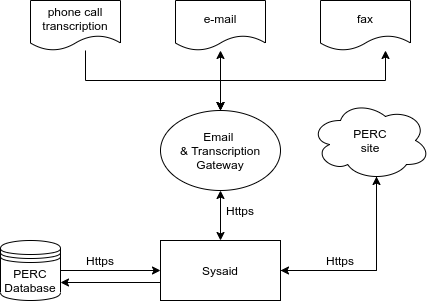
\includegraphics[width=120mm]{./img/implementations/infrastructure.png}
	\caption{High level help desk infrastructure}\label{fig:high-level-help-desk-infrastructure}
\end{figure}

\subsubsection{Sysaid Setup}\label{setup}
Giglium firmly believes in the \textit{\gls{iac}} principles, for this reason Giglium will provide a Terraform\cite{terraform} script that will create and provision two\footnote{The number of the \gls{vm} can be increased and decreased using the Terraform script to respond to high or low demand.
Giglium suggests having always two \textit{\gls{vm}}s to have a good \textit{\gls{ha}}.} \textit{Windows Server 2019} \textit{\gls{vm}}s on the Azure\cite{azure} cloud.\footnote{Azure credentials will be provided from \gls{perc}.} 
The newly created machines need to have at least 4 vCore, 8 GB RAM and 32 GB of storage\cite{sysaid_requirements} but Giglium suggests using at least the \textit{Standard-A4m-v2} tier from the Azure catalog. The Terraform script will also take care of the creation of the security group using the \textit{\gls{polp}} approach.
The Terraform script will also generate the SSH key required to enter inside the \textit{\gls{vm}}s, and it will be the only one authorized to change the state of the infrastructure. The state and all the sensitive data will be store inside the autogenerated \texttt{.tfstate} file.\gls{perc} will be responsible to store this file safely. 

Once the \gls{vm}s will be up and running, the Terraform script will call an Ansible\cite{ansible} script to finish the provisioning. This script will configure the SysAid cluster, and it will safely expose its \textit{\gls{api}}. The ansible script will also connect, using SSH, to the machine provided by \textit{\gls{perc}} to install the database. Giglium will install SQL Server 2019, for this reason, the provided machine needs to follow these requirements\cite{sql_requirements}\footnote{Giglium strongly recommended to have at least 4 GB RAM.}. All the backups for this database will be the responsibility of \gls{perc}.

\begin{figure}[ht!]
	\centering
	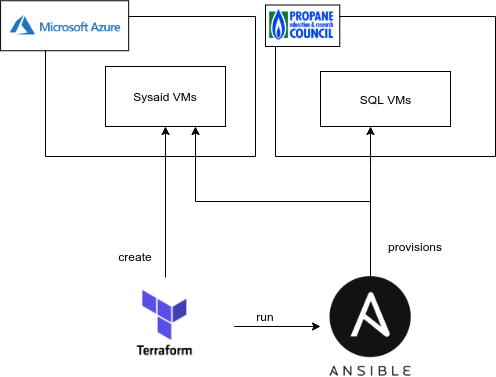
\includegraphics[width=120mm]{./img/implementations/setup.png}
	\caption{High level infrastructure set up}\label{fig:high-level-infrastructure-set-up}
\end{figure}

\paragraph{SysAid Orchestrations} To helps to automate manual, error-prone, routine tasks, Giglium will create some rules and automated actions to slash the ticket resolution time. All these configurations will be used to configure Automate Joe the native orchestrator of SysAid. Giglium will perform an initial analysis to understand the best actions to put in place. 

\paragraph{SysAid custom \textit{\gls{api}}} To connect Sysaid \textit{\gls{kb}} with the \textit{\gls{st}} Online Resource\cite{propanesafety}, Giglium will expose the Sysaid \textit{\gls{api}}. To be able to query the \textit{\gls{api}}, first of all \gls{perc} will need to login, following the procedure described here:\cite{sysaid_api_login}. Once retrieved the \texttt{JSESSIONID} token, \textit{\gls{perc}} will be able to query the following custom endpoint:

\begin{table}[h!]
	\begin{center}
		\begin{tabularx}{\linewidth}{l|X|X|}
			\toprule
			\textbf{Command Name} & \textbf{Command} & \textbf{Description}\\
			\midrule 
			Get Articles List & GET/articles?fields={field1,field2..} 
			\&offset={offset}\&limit={liqueuesmit} &  Return all articles inside the \textit{\gls{kb}}\\[10ex]
			Get Article       & GET/articles/{id}?fields={field1,field2..} & Return a specific article inside the \gls{kb}\\
			
			\bottomrule
		\end{tabularx}
		\caption{Custom \gls{api} table}\label{tab:api}
	\end{center}
\end{table}

\subsubsection{Setting up faxing in Exchange Online}\label{fax_setup}
Giglium will configure Microsoft 365 Exchange Online to receive the fax data and then sends it to SysAid with the fax included as a \texttt{.tif} attachment. Microsoft 365 Exchange Online will be also configured to receive an email composed with the main body of the email with the fax information and with attached a \texttt{.pdf} file that will be converted into the fax.

\subsubsection{Libraesva Setup}\label{libraesva_setup}
Libraesva will be our active defense against cybercrime. Giglium will configure Microsoft 365 with Libraesva as our inbound and outbound mail gateway. To be sure all the email, fax, and calls transcription will be filtered. 

\begin{figure}[ht!]
	\centering
	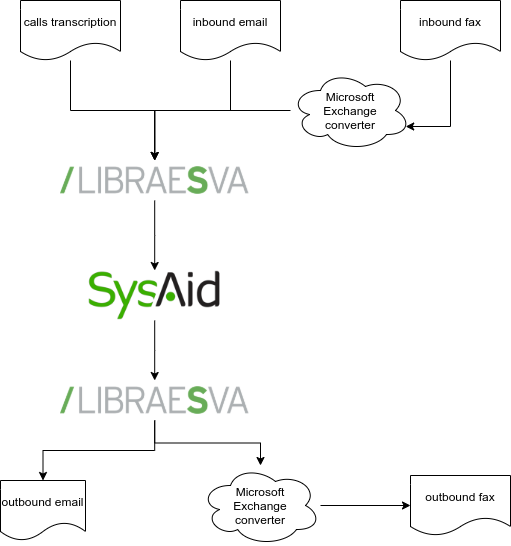
\includegraphics[width=120mm]{./img/implementations/io.png}
	\caption{Sysaid Inbound and Outbound flow}\label{fig:sysaid-flow}
\end{figure}

\subsubsection{Windows Autopilot Setup}\label{autopilot_setup}
Giglium will configure Windows autopilot to set up and pre-configure new devices or reset, repurpose, and recover devices. Windows Autopilot will:

\begin{itemize}
	\item automatically join devices to \textit{\gls{ad}};
	\item restrict the Administrator account creation;
	\item install all the necessary softwares;
\end{itemize}

\subsubsection{Microsoft 365 Teams Voice Setup}\label{365_setup}
Giglium will configure Microsoft 365 Teams Voice with a call queue that provides:

\begin{itemize}
	\item a greeting message;
	\item music while people are waiting on hold in a queue;
	\item a \textit{\gls{fifo}} call routing;
	\item some options to manage for queue overflow and timeout.
\end{itemize}

\subsection{Non-Technical Artifacts}\label{not_tecnical}
A non-technical artifacts must be configured to satisfied fulfill \textit{\gls{perc}} request. The activities, within Giglium are responsible to make in time are described in the following subsection.

\subsubsection{Help Desk User Workspace Kit}
To ensure a more flexible and cost-saving help desk, Giglium has built a strong cloud-based infrastructure. This will permit all help desk users to work from home. The minimum requirements are an internet connection and a laptop. Work from home has several benefits for business, such as:
\begin{itemize}
	\item Increased staff motivation {-} by working from home staff will feel more trusted by their employer as the working relationship isn't as closely monitored and employees are allowed a degree of autonomy to get on with their work.
	\item Financial benefits {-} savings on office space, office supplies, utility bills, and other facilities.
	\item Fewer sickness absences {–} staff are more likely to feel happier and more energized working from home and therefore less chance of their immune system is negatively impacted by burnout. Also, the fact that employees are working in isolation there is less chance of infections spreading as would be the case within an office environment.
\end{itemize}

Giglium will be responsible to put in place a workspace kit with adequate hardware. 
Every help desk operator will have the Dell laptop: \textquotedblleft New Inspiron 15 3000\cite{dellpc}\textquotedblright with 3 Years Hardware Warranty with Onsite/In-Home Service after Remote Diagnosis. The laptop specification with a CPU AMD Ryzen™ 5\cite{amdcpu} and 8 GB RAM overlap the Microsoft 365 Business Voice requirements but Giglium strongly recommended it to reduce the normal loss of performance over time.  
In combination with their laptop, the help desk user will have the Jabra headset: \textquotedblleft EVOLVE 2 40\cite{jabraheadsets}\textquotedblright. Thanks to their outstanding noise isolation and the Microsoft Team optimization and certifications they are perfect to provide high-quality calls with students. 
Inside the kit, every operator will find a \textquotedblleft work from home\textquotedblright guideline that will help them to create the perfect workspace.


\subsection{Timeline}
Giglium is proposing an aggressive yet feasible schedule for completing the Help Desk project.
The key milestones and deliverables are summarized below. All
deliverables will have a two-week approval period during which the Giglium project
team will address any deficiencies or concerns. Following the approval, \textit{\gls{perc}} will be invoiced for each new requisites.
\bigskip


\begin{table}[H]
	\begin{ganttchart}[vgrid={draw=none, dotted}]{1}{18}
		\gantttitlelist{1,2,3}{6} \\
		\ganttgroup{Technical Artifacts}{1}{18} \\
		\ganttbar[name=svms]{Sysaid \gls{vm} Setup}{1}{12} \\
		\ganttbar[name=soc]{Sysaid Orchestrations Setup}{14}{18} \\
		\ganttbar[name=sapi]{Sysaid \gls{api} Setup}{14}{18} \\
		\ganttlink{svms}{soc}
		\ganttlink{svms}{sapi}
		
		\ganttbar[name=was]{Windows Autopilot Setup}{1}{12} \\
		\ganttbar[name=mtvs]{Microsoft 365 Teams Voice Setup}{14}{18} \\
		\ganttbar[name=ls]{Libraesva Setup}{14}{18} \\
		\ganttbar[name=feo]{Setting up faxing in Exchange Online}{14}{18} \\
		\ganttlink{was}{mtvs}
		\ganttlink{was}{ls}
		\ganttlink{was}{feo}
		
		\ganttgroup{Non-Technical Artifacts}{1}{18} \\
		\ganttbar{Help Desk User Workspace Kit}{1}{18} \\
	\end{ganttchart}
	\caption{Macro-plane chart}\label{tab:gantt}
\end{table}

In the chart~\ref{tab:gantt} we can find the macro-plane, divided into weeks. As we can see three weeks are necessary to have the whole help desk project configured. The macro plan will be more detailed and possibly modified by the Project Manager after the sign of the proposal.

\subsection{Service Delivery}
For the delivery of the help desk product described in this section, the delivery of the
service will take place according to the \textit{\gls{raci}} table~\ref{tab:i_sd_raci}.

\paragraph{Table legend:}
\begin{itemize}
	\item Responsible (\textbf{R}): executor of the activity;
	\item Accountable (\textbf{A}): responsible for the result of the activity;
	\item Consulted (\textbf{C}): provides input
	\item Informed (\textbf{I}): informed on the execution of the activity.
\end{itemize}

\begin{table}[H]
	\centering
	\begin{tabular}{|l|l|l|l|} 
		\hline
		\textbf{Activity} & \textbf{Type} & \textbf{Giglium} & \textbf{\gls{perc}}   \\
		\hline
		Architecture Definition & Architecture & A-R  &  C  \\
		\hline
		Architecture Provisionin & Infrastructure & A-R & I  \\
		\hline
		SQL Server \textit{\gls{vm}} creation & Infrastructure & C & A-R  \\
		\hline
		Azure \textit{\gls{vm}} creation & Infrastructure & A-R & C  \\
		\hline
		Azure \textit{\gls{vm}} scale up or down & Infrastructure & A-R & C  \\
		\hline
		\textit{\gls{vm}} Provisioning script & Software & A-R & I \\
		\hline 
		Firewall setup & Software & A-R & C \\
		\hline 
		Microsoft 365 Teams Voice and Fax setup & Software & A-R & I \\
		\hline 
		Sysaid setup & Software & A-R & I \\
		\hline 
		Windows Autopilot Setup & Software & A-R & I \\
		\hline 
		Libraesva Setup & Software & A-R & I \\
		\hline 
		Minor Software patch & Software & A-R & C \\
		\hline 
		Minor Windows update & Software & A-R & C \\
		\hline 
		Integration with \textit{\gls{st}} Online Resource & Software & C & A-R \\
		\hline
		SQL Server Database Backup & System & C & A-R \\
		\hline 
		Terraform \texttt{.tfstate} file safety & System & C & A-R \\
		\hline 
		Disaster Recovery Plan & System & C & A-R \\
		\hline 
		System Monitoring for SQL Server \textit{\gls{vm}} & System & C & A-R \\
		\hline 
		System Monitoring for Azure \textit{\gls{vm}} & System & A-R & I \\
		\hline 
		Help Desk User Workspace Kit & Hardware & A-R & I \\
		\hline
	\end{tabular}
	\caption{Implementations service delivery \textit{\gls{raci}}}\label{tab:i_sd_raci}
\end{table}
\clearpage
\section{Help Desk structure}\label{structure}
Understanding and optimizing the help desk organizational structure is an important critical success factor in achieving team and company goals.

\subsection{Structure}
Giglium will adapt the simple structure of Mintzberg\cite{mintzberg_book} to define the internal structure of the Help desk. This structure will rotate around the figure of the help desk coordinator, thanks to this fact, in the working group there is a flexible division of labor and activities. This structure is formed by the strategic apex (the help desk coordinator), which is its most important component, and by the operative core (the help desk operators), whose number will be defined in the subsections below.

\begin{figure}[h!]
	\centering
	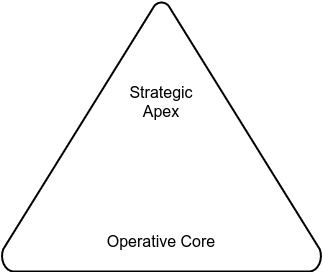
\includegraphics[width=90mm]{./img/structures/piramid.png}
	\caption{The simple structure of Mintzberg}\label{fig:piramid}
\end{figure}

The work is directly controlled by the help desk coordinator, in which there is a strong centralization of the decision-making power. This centralization allows quick decisions through an informal decision-making process. The internal relations of the working group are not institutionalized and most of the exchange information takes place between the strategic apex and the operational core. Each role represents a functional unit where it has its own functions to perform. This structure adapts easily to a simple and dynamic environment. In fact, few people would have difficulty in acting in a complex and bureaucratic environment, and, on the other hand, is a good approach to a dynamic environment. In any case, if there is no strategic apex on duty, a replacement will be temporarily appointed from the operative core.

\subsection{Kind}
\textit{\gls{perc}} has stated that it wants to release the e-lerning program on a state-by-state basis over several months. For this reason, Giglium predicts that out of the estimated two hundred and fifty copies per state sold in the first month of release, an initial service desk worker ratio of $4:250$ equal to coverage of 1.6\%. Giglium will illustrate the possible kind to suit the \textit{\gls{perc}} needs.

\subsubsection{Kind 12{-}5}\label{12_5}
To build a help desk that offers twelve hours of service (9:00 \textit{\gls{am}} to 9:00 \textit{\gls{pm}} \textit{\gls{etz}}) five days a week, Giglium recommends the following staff:
\begin{itemize}
	\item a total of two help desk coordinators;
	\item a total of six help desk operators.
\end{itemize}

\noindent Staff shifts will take place according to the table~\ref{tab:shifts_12_5}.

\paragraph{Table~\ref{tab:shifts_12_5} legend:}
\begin{itemize}
	\item Morning (\textbf{M}): from 9:00 \textit{\gls{am}} to 03:00 \textit{\gls{pm}} \textit{\gls{etz}};
	\item Afternoon (\textbf{A}): from 03:00 \textit{\gls{pm}} to 09:00 \textit{\gls{pm}} \textit{\gls{etz}};
	\item Rest (\textbf{R}): day of rest;
	\item Operator (\texttt{OP}): the help desk operator plus an identification number;
	\item Coordinator (\texttt{C}): the help desk coordinator plus an identification number.
\end{itemize}

\begin{table}[H]
	\centering
	\begin{tabular}{|l|c|c|c|c|c|c|c|c|} 
		\hline
		& \textbf{Day 1} & \textbf{Day 2} & \textbf{Day 3} & \textbf{Day 4} & \textbf{Day 5} & \textbf{Day 6} & \textbf{Day 7} & \textbf{Hours per week}\\ 
		\hline
		\texttt{C1} & M & A & M & A & A & R & R & 30\\
		\hline
		\texttt{C2} & A & M & A & M & M & R & R & 30\\
		\hline
		\texttt{OP1} & M & M & M & M & M & R & R & 30\\
		\hline
		\texttt{OP2} & A & A & A & A & A & R & R & 30\\
		\hline
		\texttt{OP3} & M & M & M & M & M & R & R & 30\\
		\hline
		\texttt{OP4} & A & A & A & A & A & R & R & 30\\
		\hline
		\texttt{OP5} & M & M & M & M & M & R & R & 30\\
		\hline
		\texttt{OP6} & A & A & A & A & A & R & R & 30\\
		\hline
	\end{tabular}
	\caption{Help desk kind 12{-}5 shifts matrix}\label{tab:shifts_12_5}
\end{table}

\subsubsection{Kind 12{-}7}\label{12_7}
To build a help desk that offers twelve hours of service (9:00 \textit{\gls{am}} to 9:00 \textit{\gls{pm}} \textit{\gls{etz}}) seven days a week, Giglium recommends the following staff:
\begin{itemize}
	\item a total of three help desk coordinators;
	\item a total of eight help desk operators.
\end{itemize}

\noindent Staff shifts will take place according to the table~\ref{tab:shifts_12_7}.

\paragraph{Table~\ref{tab:shifts_12_7} legend:}
\begin{itemize}
	\item Morning (\textbf{M}): from 09:00 \textit{\gls{am}} to 03:00 \textit{\gls{pm}} \textit{\gls{etz}};
	\item Afternoon (\textbf{A}): from 03:00 \textit{\gls{pm}} to 09:00 \textit{\gls{pm}} \textit{\gls{etz}};
	\item Rest (\textbf{R}): day of rest;
	\item Operator (\texttt{OP}): the help desk operator plus an identification number;
	\item Coordinator (\texttt{C}): the help desk coordinator plus an identification number.
\end{itemize}

\begin{table}[H]
	\centering
	\begin{tabular}{|l|c|c|c|c|c|c|c|c|} 
		\hline
		& \textbf{Day 1} & \textbf{Day 2} & \textbf{Day 3} & \textbf{Day 4} & \textbf{Day 5} & \textbf{Day 6} & \textbf{Day 7} & \textbf{Hours per week}\\ 
		\hline
		\texttt{C1} & A & M & A & M & A & R & R & 30\\
		\hline
		\texttt{C2} & M & A & M & R & R & M & A & 30\\
		\hline
		\texttt{C3} & A & R & R & A & M & A & M & 30\\
		\hline
		\texttt{OP1} & M & A & M & A & M & R & M & 36\\
		\hline
		\texttt{OP2} & A & M & A & M & R & R & A & 30\\
		\hline
		\texttt{OP3} & M & A & M & R & R & A & M & 30\\
		\hline
		\texttt{OP4} & A & M & R & R & A & M & A & 30\\
		\hline
		\texttt{OP5} & M & R & R & A & M & A & M & 30\\
		\hline
		\texttt{OP6} & R & R & A & M & A & M & A & 30\\
		\hline
		\texttt{OP7} & R & M & M & A & M & A & R & 30\\
		\hline
		\texttt{OP8} & R & A & A & M & A & M & R & 30\\
		\hline
	\end{tabular}
	\caption{Help desk kind 12{-}7 shifts matrix}\label{tab:shifts_12_7}
\end{table}

\subsubsection{Kind 24{-}5}\label{24_5}
To build a help desk that offers twenty-four hours of service (0:00 \textit{\gls{am}} to 0:00 \textit{\gls{am}} \textit{\gls{etz}}) five days a week, Giglium recommends the following staff:
\begin{itemize}
	\item a total of three help desk coordinators;
	\item a total of eight help desk operators.
\end{itemize}

\noindent Staff shifts will take place according to the table~\ref{tab:shifts_24_5}.

\paragraph{Table~\ref{tab:shifts_24_5} legend:}
\begin{itemize}
	\item Morning (\textbf{M}): from 07:00 \textit{\gls{am}} to 03:00 \textit{\gls{pm}} \textit{\gls{etz}};
	\item Afternoon (\textbf{A}): from 03:00 \textit{\gls{pm}} to 11:00 \textit{\gls{pm}} \textit{\gls{etz}};
	\item Night (\textbf{N}): from 11:00 \textit{\gls{pm}} to 07:00 \textit{\gls{am}} \textit{\gls{etz}};
	\item Rest (\textbf{R}): day of rest;
	\item Operator (\texttt{OP}): the help desk operator plus an identification number;
	\item Coordinator (\texttt{C}): the help desk coordinator plus an identification number.
\end{itemize}

\begin{table}[H]
	\centering
	\begin{tabular}{|l|c|c|c|c|c|c|c|c|} 
		\hline
		& \textbf{Day 1} & \textbf{Day 2} & \textbf{Day 3} & \textbf{Day 4} & \textbf{Day 5} & \textbf{Day 6} & \textbf{Day 7} & \textbf{Hours per week}\\ 
		\hline
		\texttt{C1} & M & A & M & A & A & R & R & 40\\
		\hline
		\texttt{C2} & A & M & A & M & M & R & R & 40\\
		\hline
		\texttt{C2} & N & N & N & N & N & R & R & 40\\
		\hline
		\texttt{OP1} & M & M & M & M & M & R & R & 40\\
		\hline
		\texttt{OP2} & A & A & A & A & A & R & R & 40\\
		\hline
		\texttt{OP3} & M & M & M & M & M & R & R & 40\\
		\hline
		\texttt{OP4} & A & A & A & A & A & R & R & 40\\
		\hline
		\texttt{OP5} & M & M & M & M & M & R & R & 40\\
		\hline
		\texttt{OP6} & A & A & A & A & A & R & R & 40\\
		\hline
		\texttt{OP7} & N & N & N & N & N & R & R & 40\\
		\hline
		\texttt{OP8} & N & N & N & N & N & R & R & 40\\
		\hline
	\end{tabular}
	\caption{Help desk kind 24{-}5 shifts matrix}\label{tab:shifts_24_5}
\end{table}

\begin{tcolorbox}
	During the night shift, Giglium expects far fewer users than the other shifts for this the initial service desk worker ratio will be reduced to $3:250$ equal to coverage of 1.2\%.
\end{tcolorbox}

\subsubsection{Kind 24{-}7}\label{24_7}
To build a help desk that offers twenty-four hours of service (0:00 \textit{\gls{am}} to 0:00 \textit{\gls{am}} \textit{\gls{etz}}) seven days a week, Giglium recommends the following staff:
\begin{itemize}
	\item a total of five help desk coordinators;
	\item a total of ten help desk operators.
\end{itemize}

\noindent Staff shifts will take place according to the table~\ref{tab:shifts_24_7}.

\paragraph{Table~\ref{tab:shifts_24_7} legend:}
\begin{itemize}
	\item Morning (\textbf{M}): from 07:00 \textit{\gls{am}} to 03:00 \textit{\gls{pm}} \textit{\gls{etz}};
	\item Afternoon (\textbf{A}): from 03:00 \textit{\gls{pm}} to 11:00 \textit{\gls{pm}} \textit{\gls{etz}};
	\item Night (\textbf{N}): from 11:00 \textit{\gls{pm}} to 07:00 \textit{\gls{am}} \textit{\gls{etz}};
	\item Rest (\textbf{R}): day of rest;
	\item Operator (\texttt{OP}): the help desk operator plus an identification number;
	\item Coordinator (\texttt{C}): the help desk coordinator plus an identification number.
\end{itemize}

\begin{table}[H]
	\centering
	\begin{tabular}{|l|c|c|c|c|c|c|c|c|} 
		\hline
		& \textbf{Day 1} & \textbf{Day 2} & \textbf{Day 3} & \textbf{Day 4} & \textbf{Day 5} & \textbf{Day 6} & \textbf{Day 7} & \textbf{Hours per week}\\ 
		\hline
		\texttt{C1} & A & M & A & M & A & R & R & 40\\
		\hline
		\texttt{C2} & M & A & M & R & R & M & A & 40\\
		\hline
		\texttt{C3} & A & R & R & A & M & A & M & 40\\
		\hline
		\texttt{C4} & N & N & N & N & R & R & N & 40\\
		\hline
		\texttt{C5} & N & N & R & R & N & N & N & 40\\
		\hline
		\texttt{OP1} & M & A & M & A & M & R & R & 40\\
		\hline
		\texttt{OP2} & A & M & A & M & R & R & A & 40\\
		\hline
		\texttt{OP3} & M & A & M & R & R & A & M & 40\\
		\hline
		\texttt{OP4} & A & M & R & R & A & M & A & 40\\
		\hline
		\texttt{OP5} & M & R & R & A & M & A & M & 40\\
		\hline
		\texttt{OP6} & R & R & A & M & A & M & A & 40\\
		\hline
		\texttt{OP7} & R & M & M & A & M & A & R & 40\\
		\hline
		\texttt{OP8} & R & A & A & M & A & M & R & 40\\
		\hline
		\texttt{OP9} & N & R & N & N & N & N & R & 40\\
		\hline
		\texttt{OP10} & R & N & N & N & N & R & M & 40\\
		\hline
	\end{tabular}
	\caption{Help desk kind 12{-}7 shifts matrix}\label{tab:shifts_24_7}
\end{table}

\begin{tcolorbox}
	During the night shift, Giglium expects far fewer users than the other shifts for this, the initial service desk worker ratio will be reduced to $3:250$ equal to coverage of 1.2\%. 
	
	During the night shift on weekends, Giglium expects even fewer users than the night shift and for this the initial service desk employment ratio will be reduced to $2:250$ equal to coverage of 0.8\%.
\end{tcolorbox}

\subsection{Management of working hours and shifts}
The help desk coordinators are responsible for scheduling the shifts which must comply with the contractual obligation hours and be consistent with the established service hours. The same are required to draw up and present the monthly hourly prospectuses of the operators distributed on several shifts, by the 25th of the previous month. These shifts may vary according to the availability of staff (holidays, daily leave, and sickness) and it will be the responsibility of the help desk coordinator to promptly notify \textit{\gls{perc}} of any changes.

The main criteria for scheduling working hours and shifts are described in the following bullet:
\begin{itemize}
	\item in the case of kind 12{-}5 (see: section~\ref{12_5}) or 12{-}7 (see: section~\ref{12_7}) the average duration of the working hours cannot exceed 40 hours every seven days (including extraordinary), since all the help desk coordinator and operators have a part-time contract;
	\item in the case of kind 24{-}5 (see: section~\ref{24_5}) or 24{-}7 (see: section~\ref{24_7}) the average duration of the working hours cannot exceed 48 hours every seven days (including extraordinary), since all the help desk coordinator and operators have a full-time contract;
	\item if the daily working hours exceed 6 hours, the worker has the right to a lasting break
	not less than 10 minutes;
	\item Each worker must benefit, over a period of 24 hours, in no less than 11 consecutive hours of daily rest;
	\item the night period is a period of at least seven consecutive hours including the interval between midnight and five in the morning (from 00:00 \textit{\gls{am}} at 5:00 \textit{\gls{pm}} \textit{\gls{etz}}). Specific suitability for night work is ascertained through the Competent Doctor. A worker without the doctor approval cannot perform any night shifts;
	\item a help desk coordinator need to be always available. In any case, if there is no help desk coordinator on duty, a replacement will be temporarily appointed from the operators;
	\item the initial service desk ratio are indicative and not binding to be manteing to be manteing.
\end{itemize}
\clearpage
\section{Procedures}\label{procedures}
Responding to service requests/incidents, generally, is not a simple matter. Service request management and incident management and response activities require knowledge, communication, and coordination among all the people that have to
respond to the service request/incident. Accordingly, the goals of this plan are:
\begin{enumerate}
	\item provides high-quality customer service and results;
	\item responding, systematically, following proven procedures, which will be saving time and money;
	\item minimizing the impact on the interest and honor of \textit{\gls{perc}}.
\end{enumerate}

\subsection{Purpose}\label{purpose}	
This document describes the	overall plan for responding to requests/incidents regarding the e-learning Certified Employee Training Program distributes by \textit{\gls{perc}}. It defines the roles and responsibilities of all the participants with the goal of detecting and react to incidents, determines their scope and risk, responds appropriately to the incident, communicates the results and the risk to all stakeholders, and reduces the likelihood of the incident from reoccurring.

\subsection{Audience}	
  
This plan applies to the call center operators and any person who gains access to SysAid.	
  	
\subsection{Maintenance}  
Giglium is responsible for the maintenance and revision of this document, with the help of \textit{\gls{perc}}.

\subsubsection{Definitions}
The following definitions are used in the next sections:
\begin{itemize}
	\item \textbf{Service request} is a formal request from a user for something to be provided. For example, a request for information or advice.	
	
	\item \textbf{Incidents} is any event that is not part of the standard operation of the \gls{perc} e-learning Certified Employee Training Program service and which causes an interruption or a reduction in quality of the service.
	
	\item \textbf{Workaround} is a temporary fix to an incident or sequence of actions alternative to the one that produces the accident, usable by the final user.
	
	\item \textbf{Personal Information} is the combination of a person’s first name (or initial) and surname, in combination with any of the following:
	\begin{itemize}
		\item social security number;
		\item driver’s license number;
		\item state identification card number;
		\item financial account, debit, or credit number;
	\end{itemize}
\end{itemize}

\subsection{Service Requests Management}
Giglium recommends that service request management have to be managed through a process. This process includes a number of sub-processes that accompany the request from the submission through its closure, where continuous monitoring, tracking, and communication are involved throughout each step. Giglium strongly suggests these sub-processes:
\begin{enumerate}
	\item service request submitted;
	\item service request assessed;
	\item service request fulfilled;
	\item service request closed.
\end{enumerate}

\begin{figure}[h!]
	\centering
	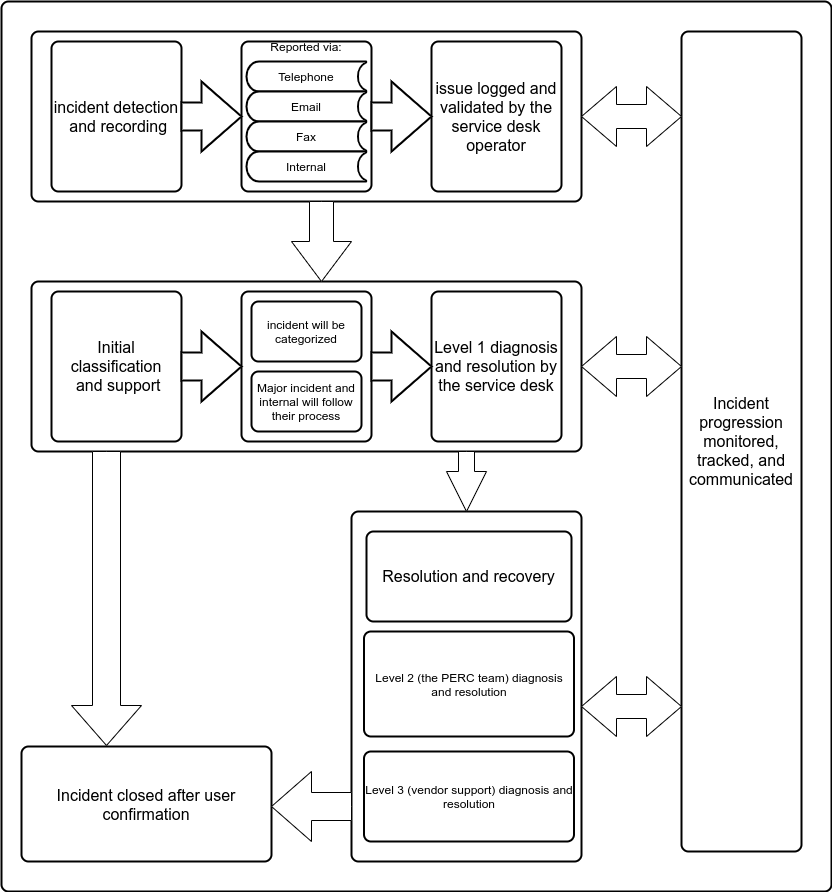
\includegraphics[width=120mm]{./img/procedures/incident-workflow.png}
	\caption{Service request management process}\label{fig:request-wrokflow}
\end{figure}

\subsubsection{Service Request Submitted}
Users can submit a request for service by:
\begin{itemize}
	\item \textbf{Telephone}: the help desk can be notified by calling them at 1 (800) XXXX\footnote{The real telephone number will be defined after the sign of the proposal. But the toll-free number 1 (800) will be preserved.\label{fnlabel}}.
	
	\item \textbf{Email and fax}: the help desk can be notified by sending an email at \href{mailto:info@propanesafety.com}{info@propanesafety.com} or by fax at 1 (800) XXXX\footref{fnlabel}.
\end{itemize}
On the first contact, a ticket is automatically open in the service request section of SysAid.

\subsubsection{Service Request Assessed}
The Help Desk team must first assess the request before any actions are taken to fulfill it. The operator will compile all the fields on the SysAid’s Service Request management triage page to classify the service request. If the information provided by the user isn't enough to fulfill the service request it will ask for more information. During this phase, the operator will assign a priority following the table~\ref{tab:request-priority}.

\begin{table}[H]
	\centering
	\begin{tabular}{ | l | l | l | l | l | }
		\cline{3-5}
		\multicolumn{2}{c|}{}& \multicolumn{3}{|c|}{Impact}  \\ \cline{3-5}
		\multicolumn{2}{c|}{} &Low & Medium  & High \\ \hline
		\multirow{3}{*}{\rotatebox{90}{\tiny Urgency\,}} & Low & \cellcolor{green}Low & \cellcolor{yellow}Medium & \cellcolor{red}High\\ \cline{2-5}
		&   Medium & \cellcolor{yellow}Medium & \cellcolor{yellow}Medium & \cellcolor{red}High \\ \cline{2-5}
		&  High & \cellcolor{red}High & \cellcolor{red}High & \cellcolor{red}High \\ \hline
	\end{tabular}
	\captionof{table}{Service request priority matrix}\label{tab:request-priority}
\end{table}
\gls{perc} and Giglium they expect most requests to be a request for information, concerning:
\begin{itemize}
	\item Installation questions (on individual work stations or across an Intranet);
	\item DVD activation questions (where to find the key code or looking up a missing key code in
	the key code database);
	\item Navigation questions (how to navigate through the interface);
	\item File sharing questions (how to locate and transfer a student record flat file);
	\item General troubleshooting;
	\item questions and issue about the “time bomb”.
\end{itemize}

For this request of information application-specific training and scripts for the operators will be provided by \gls{perc}. They required that the Help Desk personnel will not support the following types of questions, but it will be provided with a script on where to refer users:
\begin{itemize}
	\item Content-related questions;
	\item Identification of Certified Employee Training Program instructors;
	\item Certification/examination issues;
	\item Advanced network-specific questions.
\end{itemize}

Since a request for information doesn't require any planning or approval they are fulfilled during the service request assessed sub-process, from the help desk operator. The operator will simply respond by following the instructions received from \textit{\gls{perc}}, and it will found them inside the SysAid \textit{\gls{kb}}.

\begin{tcolorbox}
	If during the Service request assessed the operator believes that the service request is an incident it has to follow the incident management process describe at~\ref{incident}.
\end{tcolorbox}

\subsubsection{Service Request Fulfilled}
\gls{perc} required that all the requests for service, that are not requesting for information, have to be approved by a supervisor of the related competence area. The operator will put this request in the wait for approval state on SysAid and the system will automatically assign the ticket to the right person, notify it by email. The approver needs to provide a supply list, estimated time for completion, and the instruction so the operator can complete the request satisfactorily.

\subsubsection{Service request closed}
The importance of post-service request fulfillment activities is often underestimated. The ticket is maintained in SysAid since they provide key data such as the overall \textit{\gls{mttr}} tickets and each operator's \textit{\gls{mttr}}. They also contribute to workflow analysis to improve the service request process. The operator will also send a survey to the users who open the request for service to ask for feedback.

\subsubsection{Service Catalog}
Giglium will not implement any service catalog because \textit{\gls{perc}} it will create a comprehensive online service catalog, based on the history of previous service requests registered on SysAid by querying the custom \textit{\gls{api}}~(for \textit{\gls{api}} info see section~\ref{setup}).

\clearpage
\subsection{Incident Management}\label{incident}
Giglium recommends that incidents have to be managed through a process. This process includes a number of sub-processes that accompany the incident from the initial identification or reporting through its resolution and the closure, where continuous monitoring, tracking, and communication are involved throughout each step. Giglium strongly suggests these sub-processes:
\begin{enumerate}
	\item incident detection and recording;
	\item initial classification and support;
	\item investigation and diagnosis;
	\item resolution and recovery;
	\item incident closure.
\end{enumerate}

\begin{figure}[ht!]
	\centering
	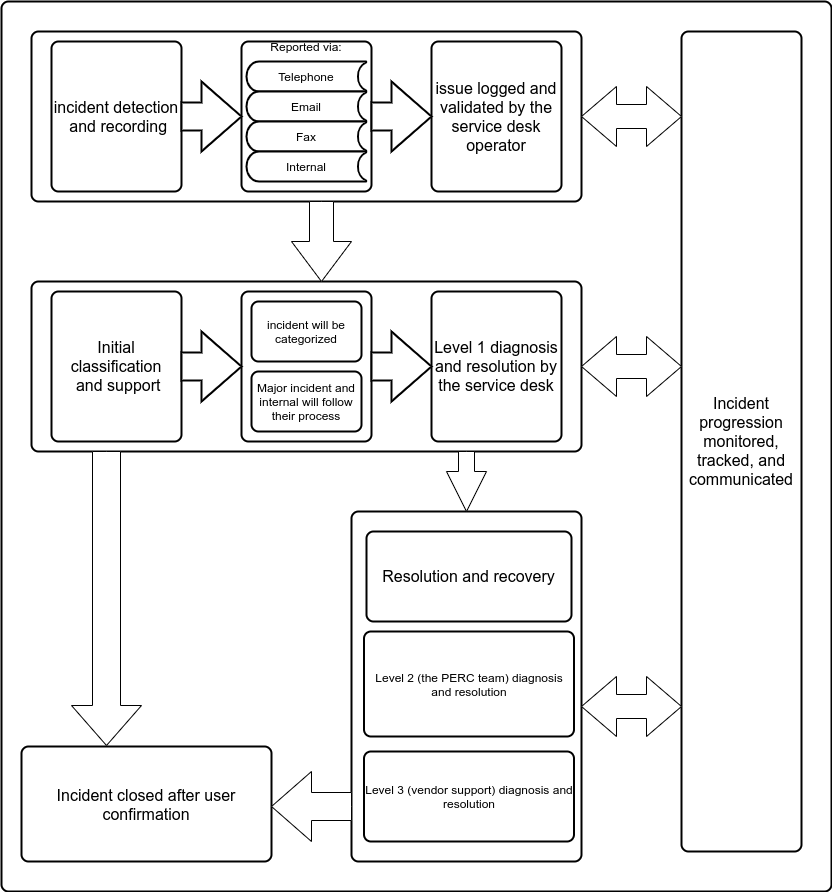
\includegraphics[width=120mm]{./img/procedures/incident-workflow.png}
	\caption{Incident Management Process}\label{fig:incident-wrokflow}
\end{figure}

\subsubsection{Incident detection and recording}
An incident can arrive from the following sources:
\begin{itemize}
	\item \textbf{Telephone, email, and fax}: during the Service request assessed phase if the operator believes that the service request is an incident it will open an incident ticket. The operator will ask the following questions to verify and collect all the information regarding the incident:
	\begin{itemize}
		\item Who is calling? Name and Title?
		\item What is their contact phone number or email address?
		\item What is the DVD key code?
		\item What is the disservice he encounters?
	\end{itemize}
	
	\item \textbf{Internal}: For internal use only. Sometimes the SysAid user can found some incident that impacts his works or the service. In this case, we will track this event with the opening of a ticket and we will process it with a specific workflow. 
\end{itemize}

When a ticket is open in SysAid all the designated party~(s) will be notified.

\begin{tcolorbox}
	It's important to notice that during this initial phase we will collect some users' personal information. It's very important to keep them safe and for this reason, they will be stored only inside the Database and they will be not queryable from any SysAid \textit{\gls{api}}.
\end{tcolorbox}

\subsubsection{Initial classification and support}
The operator will have the SysAid’s Incident Management tool available outlining the necessary information needed for the appropriate response and who should be alerted regarding this incident. The operator will compile all the fields on the SysAid’s Incident Management triage page to classify the incident. During this phase, the operator will assign a priority following the table~\ref{tab:incident-priority}.of the related competence area.


\begin{table}[H]
	\centering
	\begin{tabular}{ | l | l | l | l | l | }
		\cline{3-5}
		\multicolumn{2}{c|}{}& \multicolumn{3}{|c|}{Impact}  \\ \cline{3-5}
		\multicolumn{2}{c|}{} &Low & Medium  & High \\ \hline
		\multirow{3}{*}{\rotatebox{90}{\tiny Urgency\,}} & Low & \cellcolor{green}Low & \cellcolor{yellow}Medium & \cellcolor{red}High\\ \cline{2-5}
		&   Medium & \cellcolor{yellow}Medium & \cellcolor{yellow}Medium & \cellcolor{red}High \\ \cline{2-5}
		&  High & \cellcolor{red}High & \cellcolor{red}High & \cellcolor{red}High \\ \hline
	\end{tabular}
	\captionof{table}{Incident priority matrix}\label{tab:incident-priority}
\end{table}

The operator will perform an initial diagnosis and, it will consult the \textit{\gls{kb}}, to find possible incident resolution tips and how-to solutions. The scope of this initial diagnosis is to provide a workaround for the impacted user. There are two use cases that don't require any diagnosis and need to be immediately escalated:

\begin{itemize}
	\item in case of major incident \textit{\gls{perc}} required to escalate the issue to its dedicated team of experts, of the related competence area. For this reason, the operator will not perform any diagnosis and the related ticket of the incident will be assigned to the on-call person of that area. If the major incident is reported via telephone the call will be redirected to the designated on-call person; 
	\item in case of internal incident Giglium required to escalate the issue to its dedicated \textit{\gls{msp}} team. For this reason, the operator will not perform any diagnosis and the related ticket of the incident will be assigned to the on-call person. 
\end{itemize}

\subsubsection{Investigation and diagnosis}
Giglium will not detail a lot this sub-process since is a \textit{\gls{perc}} responsibility but, after an initial assessment of an incident, the ticket is assigned to the \textit{\gls{perc}} team. The scope of this team is to collect additional information and analyzed them to definitively eliminate the possible cause. In this sub-process, it can be involved even external vendors. This requires a detailed recording of the actions taken and the corresponding results. 
Giglium will keep the responsibility of the communication with all the designated party~(s).

\subsubsection{Resolution and recovery}
When the \textit{\gls{perc}} team has resolved the incident, Giglium will communicate with all the designated party~(s) to confirm the resolution. After the resolution was confirmed by the impacted user, the \textit{\gls{perc}} team, will be responsible to update the \textit{\gls{kb}}. After the update, the operator that opens the ticket will review the new solution to con-validate it.

\subsubsection{Incident closure}
The ticket is closed on SysAid and all the designated party~(s) will be notified.

\subsection{Service Delivery}
For the delivery of the help desk product described in this section, the delivery of the
service will take place according to the \textit{\gls{raci}} table~\ref{tab:p_sd_raci}.

\paragraph{Table legend:}
\begin{itemize}
	\item Responsible (\textbf{R}): executor of the activity;
	\item Accountable (\textbf{A}): responsible for the result of the activity;
	\item Consulted (\textbf{C}): provides input
	\item Informed (\textbf{I}): informed on the execution of the activity.
\end{itemize}

\begin{table}[H]
	\centering
	\begin{tabular}{|l|l|l|l|} 
		\hline
		\textbf{Activity} & \textbf{Giglium} & \textbf{\gls{perc}}   \\
		\hline
		Maintenance and revision the procedures & A-R  &  C  \\
		\hline
		Level 1 support & A-R & C \\
		\hline
		Level 2 support & I & A-R \\
		\hline
		Internal incident L2 support & A-R & C \\
		\hline
		Update the \textit{\gls{kb}} & C & A-R\\
		\hline
		Review the \textit{\gls{kb}} & A-R & C\\
		\hline		
		Service catalog management & C & A-R \\
		\hline
	\end{tabular}
	\caption{Procedures service delivery \textit{\gls{raci}}}\label{tab:p_sd_raci}
\end{table}
\clearpage
\section{Cost}\label{cost}
To realize the vision that Giglium has for the \textit{\gls{perc}}'s help desk it is necessary to analyze different types of costs:
\begin{enumerate}
	\item technical artifacts;
	\item non-technical artifacts;
	\item help desk coordinator;
	\item help desk operator.
\end{enumerate}

\subsubsection{Technical Artifacts Cost}
The cost of implementing all the artifacts described in section~\ref{technical} are collected in the table~\ref{tab:tecnical_cost}.

\begin{table}[H]
	\centering
	\begin{tabular}{|l|c|c|c|} 
		\hline
		\textbf{Item} & \textbf{Unit cost} & \textbf{Discount} & \textbf{Final cost}   \\
		\hline
		\multicolumn{4}{|l|}{\textbf{1 Technical Artifacts} (see:~\ref{technical})}\\
		\hline
		\hspace{2mm}1.1 SysAid setup & \$10,000 & 20\% & \$8,000\\
		\hline
		\hspace{4mm}1.1.1 SysAid Orchestrations & \$0 & 0\% & \$0 (included in 1.1)\\
		\hline
		\hspace{4mm}1.1.2 Sysaid custom \textit{\gls{api}} & \$0 & 0\% & \$0 (included in 1.1)\\
		\hline
		\hspace{4mm}1.1.3 Maintenance	& \$0 & 0\% & \$0 (included in 1.1)\\
		\hline
		\hspace{4mm}1.1.4 Host the source code on Github & \$0 & 0\% & \$0 (included in 1.1)\\
		\hline
		\hspace{2mm}1.2 Setting up faxing Exchange Online (see:~\ref{fax_setup})  & \$150 & 0\% & \$150\\
		\hline
		\hspace{2mm}1.3 Libraesva setup (see:~\ref{libraesva_setup})  & \$2,000 & 10\% & \$1,800\\
		\hline
		\hspace{4mm}1.3.1 Libraesva license  & \$0 & 0\% & \$0 (included in 1.3)\\
		\hline
		\hspace{4mm}1.3.2 24-hour support from Libraesva  & \$0 & 0\% & \$0 (included in 1.3)\\
		\hline
		\hspace{2mm}1.4 Windows autopilot setup (see:~\ref{autopilot_setup})  & \$250 & 10\% & \$250\\
		\hline
		\hspace{4mm}1.4.1 Windows autopilot license  & \$0 & 0\% & \$0 (included in 1.4)\\
		\hline
		\hspace{2mm}1.5 Microsoft 365 setup (see:~\ref{365_setup})  & \$150 & 0\% & \$150 \\
		\hline
		\hspace{2mm}1.5 Five years Giglium technical \textit{\gls{msp}} 8{-}5  & \$500 & 25\% & \$2,000 \\
		\hline
		\multicolumn{3}{|l|}{\textbf{Total}:} & \$12,350\\
		\hline
	\end{tabular}
	\caption{Technical artifacts cost}\label{tab:tecnical_cost}
\end{table}

\subsubsection{Non-Technical Artifact Cost}
The cost of implementing all the artifacts described in section~\ref{not_tecnical} are collected in the table~\ref{tab:not_tecnical_cost}.

\begin{table}[H]
	\centering
	\begin{tabular}{|l|c|c|c|} 
		\hline
		\textbf{Item} & \textbf{Unit cost} & \textbf{Discount} & \textbf{Final cost}   \\
		\hline
		\multicolumn{4}{|l|}{\textbf{2 Non-Technical Artifacts} (see:~\ref{not_tecnical})}\\
		\hline
		\hspace{2mm}2.1 Dell laptop: \textquotedblleft New Inspiron 15 3000\textquotedblright\cite{dellpc} & \$400 & 20\% & \$320\\
		\hline
		\hspace{4mm}2.1.1 Windows 10 license & \$0 & 0\% & \$0 (included in 2.1)\\
		\hline
		\hspace{4mm}2.1.2 Windows setup  & \$0 & 0\% & \$0 (included in 1.4)\\
		\hline
		\hspace{4mm}2.1.2 Three years hardware warranty	& \$150 & 0\% & \$150 \\
		\hline
		\hspace{2mm}2.2 Jabra Headset \textquotedblleft Evolve 2 40\textquotedblright\cite{jabraheadsets} & \$140 & 20\% & \$126\\
		\hline
		\hspace{4mm}2.2.1 Drive setup & \$0 & 0\% & \$0 (included in 1.4)\\
		\hline
		\hspace{2mm}2.5 Shipping  & \$7 & 0\% & \$7\\
		\hline
		\multicolumn{3}{|l|}{\textbf{Total}:} & \$603\\
		\hline
	\end{tabular}
	\caption{Non-technical artifact cost}\label{tab:not_tecnical_cost}
\end{table}

\subsubsection{Help Desk Coordinator Cost}
The cost of hire an help desk coordinator figure, for five years, are collected in the tables:
\begin{itemize}
	\item table~\ref{tab:part_time_coordinator_cost} for the part-time worker used in kind 12{-}5 (see: section~\ref{12_5}) or 12{-}7 (see: section~\ref{12_7});
	\item table~\ref{tab:full_time_coordinator_cost} for the full-time worker used in kind 24{-}5 (see: section~\ref{24_5}) or 24{-}7 (see: section~\ref{24_7}).
\end{itemize}

\begin{minipage}{15cm}
	\begin{table}[H]
		\centering
		\begin{tabular}{|l|c|c|c|} 
			\hline
			\textbf{Item} & \textbf{Unit cost} & \textbf{Discount} & \textbf{Final cost}   \\
			\hline
			\multicolumn{4}{|l|}{\textbf{3 Part-time Help Desk Coordinator}}\\
			\hline
			\hspace{2mm}3.1  Annual Salary & \$30,000 & 0\% & \$150,000\\
			\hline
			\hspace{4mm}3.1.2 Weekend compensation\footnote{Only in case of kind 12{-}7 (see: section~\ref{12_7})}& \$4500 & 0\% & \$22,500 \\
			\hline
			\hspace{2mm}3.2 SysAid license & \$20 & 10\% & \$90 \\
			\hline
			\hspace{2mm}3.3 Microsoft 365 license  & \$20 & 20\% & \$80 \\
			\hline
			\multicolumn{3}{|l|}{\textbf{Total}:} & \$150,170\\
			\hline
			\multicolumn{3}{|l|}{\textbf{Total with weekends}:} & \$172,670\\
			\hline
		\end{tabular}
		\caption{Part-time Help desk coordinator cost}\label{tab:part_time_coordinator_cost}
	\end{table}
\end{minipage}

\begin{minipage}{15cm}
	\begin{table}[H]
		\centering
		\begin{tabular}{|l|c|c|c|} 
			\hline
			\textbf{Item} & \textbf{Unit cost} & \textbf{Discount} & \textbf{Final cost}   \\
			\hline
			\multicolumn{4}{|l|}{\textbf{4 Full-time Help Desk Coordinator}}\\
			\hline
			\hspace{2mm}4.1  Annual Salary & \$40,000 & 0\% & \$200,000\\
			\hline
			\hspace{4mm}4.1.1 Nigth compensation\footnote{Only for night workers} & \$10,000 & 0\% & \$50,000 \\
			\hline
			\hspace{4mm}4.1.2 Weekend compensation\footnote{Only in case of kind 24{-}7 (see: section~\ref{24_7})}& \$6000 & 0\% & \$30,000 \\
			\hline
			\hspace{2mm}4.2 SysAid license & \$20 & 10\% & \$90 \\
			\hline
			\hspace{2mm}4.3 Microsoft 365 license  & \$20 & 20\% & \$80 \\
			\hline
			\multicolumn{3}{|l|}{\textbf{Total}:} & \$200,170\\
			\hline
			\multicolumn{3}{|l|}{\textbf{Total with weekends}:} & \$250,170\\
			\hline
			\multicolumn{3}{|l|}{\textbf{Total with nights}:} & \$230,170\\
			\hline
			\multicolumn{3}{|l|}{\textbf{Total with nights and weekends}:} & \$280,170\\
			\hline
		\end{tabular}
		\caption{full-time Help desk coordinator cost}\label{tab:full_time_coordinator_cost}
	\end{table}
\end{minipage}

\subsubsection{Help Desk Operator Cost}
The cost of hire an help desk operator figure, for five years, are collected in the tables:
\begin{itemize}
	\item table~\ref{tab:part_time_operator_cost} for the part-time worker used in kind 12{-}5 (see: section~\ref{12_5}) or 12{-}7 (see: section~\ref{12_7});
	\item table~\ref{tab:full_time_operator_cost} for the full-time worker used in kind 24{-}5 (see: section~\ref{24_5}) or 24{-}7 (see: section~\ref{24_7}).
\end{itemize}

\begin{minipage}{15cm}
	\begin{table}[H]
		\centering
		\begin{tabular}{|l|c|c|c|} 
			\hline
			\textbf{Item} & \textbf{Unit cost} & \textbf{Discount} & \textbf{Final cost}   \\
			\hline
			\multicolumn{4}{|l|}{\textbf{5 Part-time Help Desk Operator}}\\
			\hline
			\hspace{2mm}5.1  Annual Salary & \$20,000 & 0\% & \$100,000\\
			\hline
			\hspace{4mm}5.1.2 Weekend compensation\footnote{Only in case of kind 12{-}7 (see: section~\ref{12_7})}& \$2500 & 0\% & \$12,500 \\
			\hline
			\hspace{2mm}5.2 SysAid license & \$20 & 10\% & \$90 \\
			\hline
			\hspace{2mm}5.3 Microsoft 365 license  & \$20 & 20\% & \$80 \\
			\hline
			\multicolumn{3}{|l|}{\textbf{Total}:} & \$100,170\\
			\hline
			\multicolumn{3}{|l|}{\textbf{Total with weekends}:} & \$112,670\\
			\hline
		\end{tabular}
		\caption{Part-time Help desk operator cost}\label{tab:part_time_operator_cost}
	\end{table}
\end{minipage}

\begin{minipage}{15cm}
	\begin{table}[H]
		\centering
		\begin{tabular}{|l|c|c|c|} 
			\hline
			\textbf{Item} & \textbf{Unit cost} & \textbf{Discount} & \textbf{Final cost}   \\
			\hline
			\multicolumn{4}{|l|}{\textbf{6 Full-time Help Desk Operator}}\\
			\hline
			\hspace{2mm}6.1  Annual Salary & \$27,000 & 0\% & \$135,000\\
			\hline
			\hspace{4mm}6.1.1 Nigth compensation\footnote{Only for night workers} & \$7,000 & 0\% & \$35,000 \\
			\hline
			\hspace{4mm}6.1.2 Weekend compensation\footnote{Only in case of kind 24{-}7 (see: section~\ref{24_7})}& \$3000 & 0\% & \$15,000 \\
			\hline
			\hspace{2mm}6.2 SysAid license & \$20 & 10\% & \$90 \\
			\hline
			\hspace{2mm}6.3 Microsoft 365 license  & \$20 & 20\% & \$80 \\
			\hline
			\multicolumn{3}{|l|}{\textbf{Total}:} & \$135,170\\
			\hline
			\multicolumn{3}{|l|}{\textbf{Total with weekends}:} & \$150,170\\
			\hline
			\multicolumn{3}{|l|}{\textbf{Total with nights}:} & \$170,170\\
			\hline
			\multicolumn{3}{|l|}{\textbf{Total with nights and weekends}:} & \$185,170\\
			\hline
		\end{tabular}
		\caption{full-time Help desk operator cost}\label{tab:full_time_operator_cost}
	\end{table}
\end{minipage}

\subsubsection{Summary}
The cost of a five years help desk are summurized in the tables:
\begin{itemize}
	\item table~\ref{tab:12_5_cost} for kind 12{-}5 (see: section~\ref{12_5});
	\item table~\ref{tab:12_7_cost} for kind 12{-}7 (see: section~\ref{12_7});
	\item table~\ref{tab:24_5_cost} for kind 24{-}5 (see: section~\ref{24_5});
	\item table~\ref{tab:24_7_cost} for kind 24{-}7 (see: section~\ref{24_7}).
\end{itemize}

\begin{minipage}{15cm}
	\begin{table}[H]
	\centering
	\begin{tabular}{|l|c|c|c|} 
		\hline
		\textbf{Item} & \textbf{Unit cost} & \textbf{Multiplier} & \textbf{Final cost}   \\
		\hline
		\multicolumn{4}{|l|}{\textbf{Kind 12{-}5}}\\
		\hline
		\hspace{2mm}Technical Artifacts (see: table~\ref{tab:tecnical_cost}) & \$12,350 & 1 & \$12,350\\
		\hline
		\hspace{2mm}Non-Technical Artifacts (see: table~\ref{tab:not_tecnical_cost}) & \$603 & 1.5 & \$905 \\
		\hline
		\hspace{2mm}Part-time Help Desk Coordinator (see: table~\ref{tab:part_time_coordinator_cost}) & \$150,170 & 2 & \$300,340 \\
		\hline
		\hspace{2mm}Part-time Help Desk Operator (see: table~\ref{tab:part_time_operator_cost})& \$100,170 & 6 & \$601,020 \\
		\hline
		\multicolumn{3}{|l|}{\textbf{Total}:} & \$944,615\\
		\hline
	\end{tabular}
	\caption{Help Desk kind 12{-}5 final cost for five years}\label{tab:12_5_cost}
	\end{table}
\end{minipage}

\begin{minipage}{15cm}
	\begin{table}[H]
		\centering
		\begin{tabular}{|l|c|c|c|} 
			\hline
			\textbf{Item} & \textbf{Unit cost} & \textbf{Multiplier} & \textbf{Final cost}   \\
			\hline
			\multicolumn{4}{|l|}{\textbf{Kind 12{-}7}}\\
			\hline
			\hspace{2mm}Technical Artifacts (see: table~\ref{tab:tecnical_cost}) & \$12,350 & 1 & \$12,350\\
			\hline
			\hspace{2mm}Non-Technical Artifacts (see: table~\ref{tab:not_tecnical_cost}) & \$603 & 1.5 & \$905 \\
			\hline
			\hspace{2mm}Part-time Help Desk Coordinator\footnote{It works also during weekends\label{footnote:12_7_weekend}} (see: table~\ref{tab:part_time_coordinator_cost}) & \$172,670 & 3 & \$300,340 \\
			\hline
			\hspace{2mm}Part-time Help Desk Operator\footref{footnote:12_7_weekend} (see: table~\ref{tab:part_time_operator_cost})& \$112,170 & 8 & \$1,381,360 \\
			\hline
			\multicolumn{3}{|l|}{\textbf{Total}:} & \$1,694,955\\
			\hline
		\end{tabular}
		\caption{Help Desk kind 12{-}7 final cost for five years}\label{tab:12_7_cost}
	\end{table}
\end{minipage}

\begin{minipage}{15cm}
	\begin{table}[H]
		\centering
		\begin{tabular}{|l|c|c|c|} 
			\hline
			\textbf{Item} & \textbf{Unit cost} & \textbf{Multiplier} & \textbf{Final cost}   \\
			\hline
			\multicolumn{4}{|l|}{\textbf{Kind 24{-}5}}\\
			\hline
			\hspace{2mm}Technical Artifacts (see: table~\ref{tab:tecnical_cost}) & \$12,350 & 1 & \$12,350\\
			\hline
			\hspace{2mm}Non-Technical Artifacts (see: table~\ref{tab:not_tecnical_cost}) & \$603 & 1.5 & \$905 \\
			\hline
			\hspace{2mm}Full-time Help Desk Coordinator (see: table~\ref{tab:part_time_coordinator_cost}) & \$200,170 & 2 & \$400,340 \\
			\hline
			\hspace{2mm}Full-time Night Help Desk Coordinator (see: table~\ref{tab:full_time_coordinator_cost}) & \$230,170 & 1 & \$230,170 \\
			\hline
			\hspace{2mm}Full-time Help Desk Operator (see: table~\ref{tab:full_time_operator_cost})& \$135,170 & 6 & \$811,020 \\
			\hline
			\hspace{2mm}Full-time Night Help Desk Operator (see: table~\ref{tab:full_time_operator_cost})& \$170,170 & 2 & \$340,340 \\
			\hline
			\multicolumn{3}{|l|}{\textbf{Total}:} & \$1,795,125\\
			\hline
		\end{tabular}
		\caption{Help Desk kind 24{-}5 final cost for five years}\label{tab:24_5_cost}
	\end{table}
\end{minipage}

\begin{minipage}{15cm}
	\begin{table}[H]
		\centering
		\begin{tabular}{|l|c|c|c|} 
			\hline
			\textbf{Item} & \textbf{Unit cost} & \textbf{Multiplier} & \textbf{Final cost}   \\
			\hline
			\multicolumn{4}{|l|}{\textbf{Kind 24{-}7}}\\
			\hline
			\hspace{2mm}Technical Artifacts (see: table~\ref{tab:tecnical_cost}) & \$12,350 & 1 & \$12,350\\
			\hline
			\hspace{2mm}Non-Technical Artifacts (see: table~\ref{tab:not_tecnical_cost}) & \$603 & 1.5 & \$905 \\
			\hline
			\hspace{2mm}Full-time Help Desk Coordinator\footnote{It works also during weekends\label{footnote:24_7_weekend}} (see: table~\ref{tab:part_time_coordinator_cost}) & \$250,170 & 3 & \$750,510 \\
			\hline
			\hspace{2mm}Full-time Night Help Desk Coordinator\footref{footnote:24_7_weekend} (see: table~\ref{tab:full_time_coordinator_cost}) & \$560,340 & 2 & \$230,170 \\
			\hline
			\hspace{2mm}Full-time Help Desk Operator\footref{footnote:24_7_weekend} (see: table~\ref{tab:full_time_operator_cost})& \$150,170 & 8 & \$1,201,360 \\
			\hline
			\hspace{2mm}Full-time Night Help Desk Operator\footref{footnote:24_7_weekend} (see: table~\ref{tab:full_time_operator_cost})& \$185,170 & 2 & \$370,340 \\
			\hline
			\multicolumn{3}{|l|}{\textbf{Total}:} & \$2,568,635\\
			\hline
		\end{tabular}
		\caption{Help Desk kind 24{-}7 final cost for five years}\label{tab:24_7_cost}
	\end{table}
\end{minipage}

\clearpage
\renewcommand{\arraystretch}{2.7}
\section{Offer conditions}
\begin{table}[H]
	\centering 
	\begin{tabularx}{\linewidth}{|XX|}
		\hline
		\textbf{Sales Tax}  &    10\%\\
		\textbf{Billing}: & An invoice will be issued per payment  \\
		\textbf{Payment} & Deferred. A initial 20\% of the total cost at the beginning of the works. A further 30\% of the total cost upon delivery of the help desk system. The remaining 50\% of the total cost deferred over the 5-year term of the contract. \\
		\textbf{Proposal Validity Period} & \today\text{ to }December 25, 2021 \\
		\textbf{Expected delivery / fulfillment times} & They will be agreed upon receipt of the order \\
		\textbf{Duration of the contract} & 5-year\\
		
		\multicolumn{2}{|c|}{\parbox{15 cm}{The offer is considered valid in its completeness of configuration. Partial orders are not accepted.\bigskip}}\\

		\multicolumn{2}{|c|}{\parbox{15 cm}{In the event of a conflict between the clauses of the general conditions of Giglium Inc.\ and the content of the commercial offer or the general conditions of the customer always prevails the content of the former.\bigskip}}\\
		
		\multicolumn{2}{|c|}{\parbox{15 cm}{By accepting this the customer:
			\begin{itemize}
				\item Declares to be aware of the contractual conditions of use of the product and/or service purchased and declares to accept them in all their parts the general conditions of Giglium Inc.\  published on the website \url{https://www.giglium.com/general-conditions/}
				\item Authorizes the processing of the data provided which will be used by both Giglium Inc.\ that by its suppliers for the sole purpose of proper management and order fulfillment
			\end{itemize}
		}}\\

		\hline
	\end{tabularx}
\end{table}
\renewcommand{\arraystretch}{1}

\glsaddall
\clearpage
\pagenumbering{gobble}
\printglossary[type=\acronymtype]
\newpage
\printglossary[type=main]
\newpage
\bibliography{bibliographic}
\bibliographystyle{ieeetr}
\end{document}